\section{Scattered Light}
\subsection{Additional Count Rate from Arbitrary Source}
Let $s(\theta)$ be the lens hood suppression as a function of angle $\theta$ 
from the camera boresight to a given point-source on the sky. By definition,
\begin{equation}
s(\theta) \equiv \frac{F_\mathrm{obs}}{F_\mathrm{ns}},
\end{equation}
for $F_\mathrm{obs}$ the observed flux of the source (that which reaches the 
CCD), and $F_\mathrm{ns}$ the flux that would be observed with no 
suppression and $\theta=0$.
The observed flux of the source can then be written as a function of $\theta$
\begin{align}
	F_\mathrm{obs}(\theta) &= s(\theta) F_\mathrm{ns}  \\
	&= s(\theta) F_0 10^{-0.4(m_\mathrm{ns} - m_0)} ,
\end{align}
for $F_0$ the (non-suppressed) flux corresponding to a source with zero-point 
apparent magnitude $m_0$, and $m_\mathrm{ns}$ the apparent magnitude of 
the source with no suppression.
\citet{winn_searchable_2013} tabulates $F_0 = 
1.6\times10^6\,\mathrm{ph/s/cm^2}$ 
for an $I=0$, G2V star.
Thus
\begin{equation}
F_\mathrm{obs}(\theta) = (1.6\times 10^6) s(\theta) 10^{-0.4 m_\mathrm{ns}} 
\quad \mathrm{[ph/s/cm^2]}.
\end{equation}

We can then write the following expression for $\mu\equiv F_\mathrm{obs} A \eta 
/ N$, the mean incident count rate on the pixel of interest:
\begin{equation}
\mu =  (1.6\times 10^6) s(\theta) 10^{-0.4 m_\mathrm{ns}} \frac{A 
\eta}{N} \quad \mathrm{[ct/px/s]},
\end{equation}
for $A$ the effective observing area in $\mathrm{cm^2}$, $N$ the 
number of pixels per camera, and $\eta$ the quantum efficiency.
For TESS, $A=69.1\,\mathrm{cm^2}$, $N=4096^2$, and $\eta\approx 1$. Using
these numbers gives
\begin{equation}
\mu = 6.59  s(\theta) 10^{-0.4 m_\mathrm{ns}}\quad 
\mathrm{[ct/px/s]}.
\label{eq:mean_added_flux}
\end{equation}

The above expression assumes that the scattered flux from the source 
is uniformly spread across the CCD. The reality may be quite different,
but our purpose in this case is to simply get order-of-magnitude accuracy.
Another caveat is that our zero-point relies on an $I$ magnitude calibration -- 
a more accurate approach would use separate bandpass-dependent zero-points.

Assuming a Poisson arrival rate, the standard deviation in the number of counts 
per pixel per 2 second readout is then
\begin{equation}
\sigma \approx \mu^{1/2} = \left[ 13.2 s(\theta) 10^{-0.4 m_\mathrm{ns}} 
\right]^{1/2}\quad \mathrm{[ct/px\ RMS\ per\ 2\ sec\ image]}.
\label{eq:added_RMS}
\end{equation}

\subsection{Effect on  {\rm \npole}}
\label{sec:scattered_npole}
\begin{figure}[!t]
	\centering
	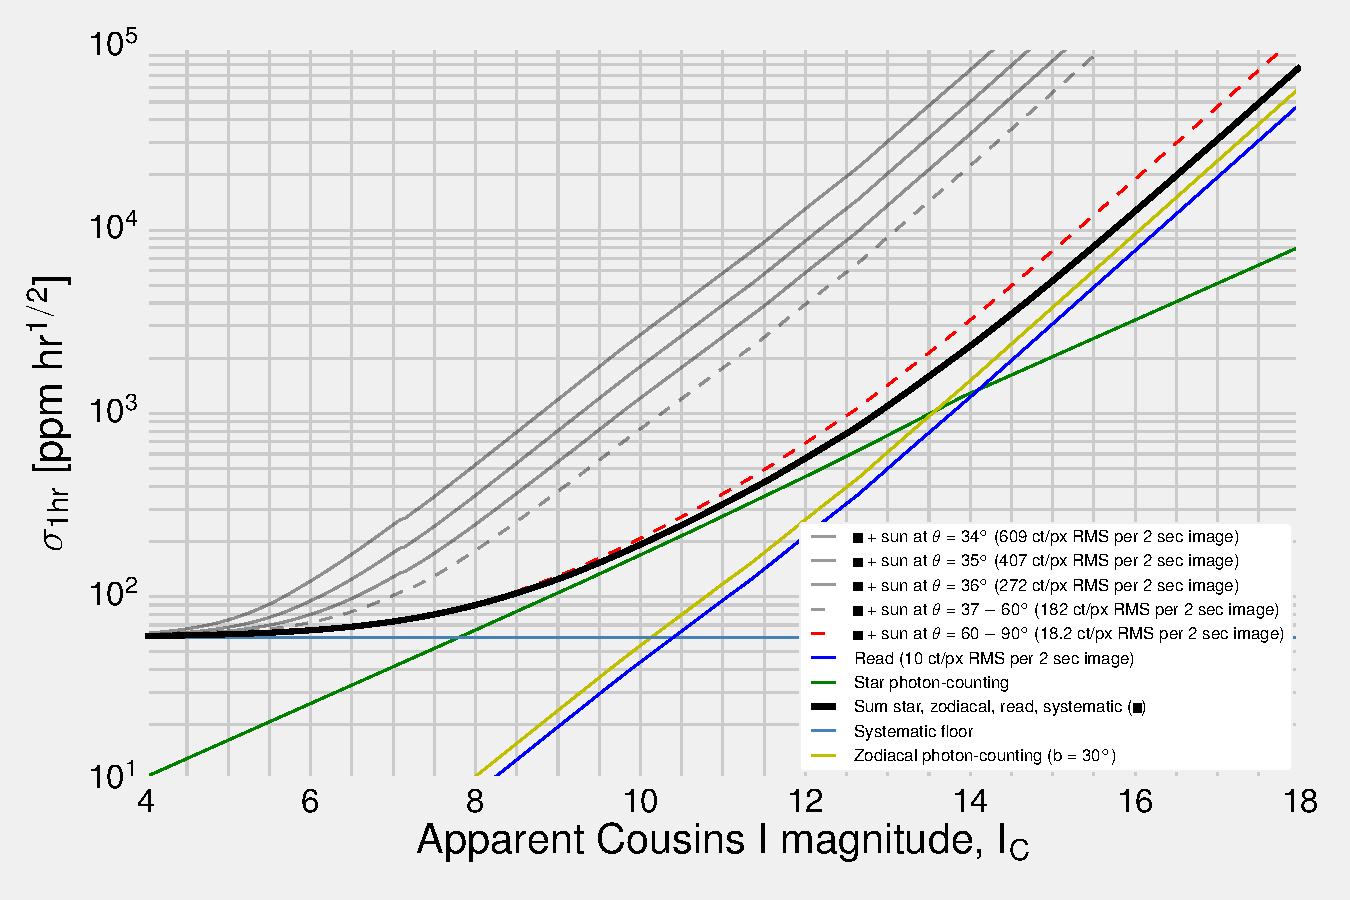
\includegraphics{figures/precision_angles_sun.pdf}
	\caption{Noise budget including Solar scattered light at different angles 
		$\theta$ from camera boresight. Note that lines where $\mu \gtrsim 
		10^5\,\mathrm{ct/px/s}$ from Eq.~\protect\ref{eq:mean_added_flux} are 
		in 
		fact 
		saturated and thus completely unusable. The lines are spaced by 
		$1^\circ$.} 
	\label{fig:sun_scat}
\end{figure}
To compute the net effect on TESS's noise budget, we add $\sigma$ from 
Eq.~\ref{eq:added_RMS} in quadrature with Eq.~\ref{eq:snr}.
We assume $m_\mathrm{ns}$ values of $-26,-13,\,\mathrm{and}\ -17.76$ for the 
Sun, Moon, and Earth respectively.
This gives Figs.~\ref{fig:sun_scat}-\ref{fig:earth_scat}.
The important point for \npole\ is shown in the dotted and dashed red lines of 
Fig.~\ref{fig:sun_scat}. 
The dotted red line corresponds to the Sun at $\theta=37-60^\circ$.
If \tess were to simply rotate $36^\circ$ about spacecraft $+Y$ 
(Fig.~\ref{fig:spacecraft_angles}) Camera 4 would be $45^\circ$
away from the Sun.
Thus it would be in the regime of the dotted red line -- likely an unacceptable 
level of background flux.

The next thing to imagine would be rotating $\zeta=90^\circ$ about spacecraft 
$+Z$, 
following the initial rotation that oriented the spacecraft in the `dotted red 
line' regime.
This puts us in the regime of the dashed red line, now for all cameras.
This is likely an acceptable level of background noise.
However, it puts one solar panel completely in the shadow of the spacecraft, 
while the other's normal would be perpendicular to incoming solar rays and thus 
unable to operate.

The middle ground would be rather than rotating all the way to 
$\zeta=90^\circ$, rotate by $\zeta = 60^\circ$, or some amount dependent on 
in-flight diagnostics of \tesss lens hood performance.
If there is a regime in which a  compromise can be reached between
power usage and scattered sunlight, it will exist near here.
Given the coarseness of our lens hood model 
(Fig.~\ref{fig:lens_hood_suppression}), we proceed in the main report as if
this problem can be addressed, and for simplicity ignore the expected
modified RMS shown in Fig.~\ref{fig:sun_scat}'s dashed red line.

 

\begin{figure}[!t]
	\centering
	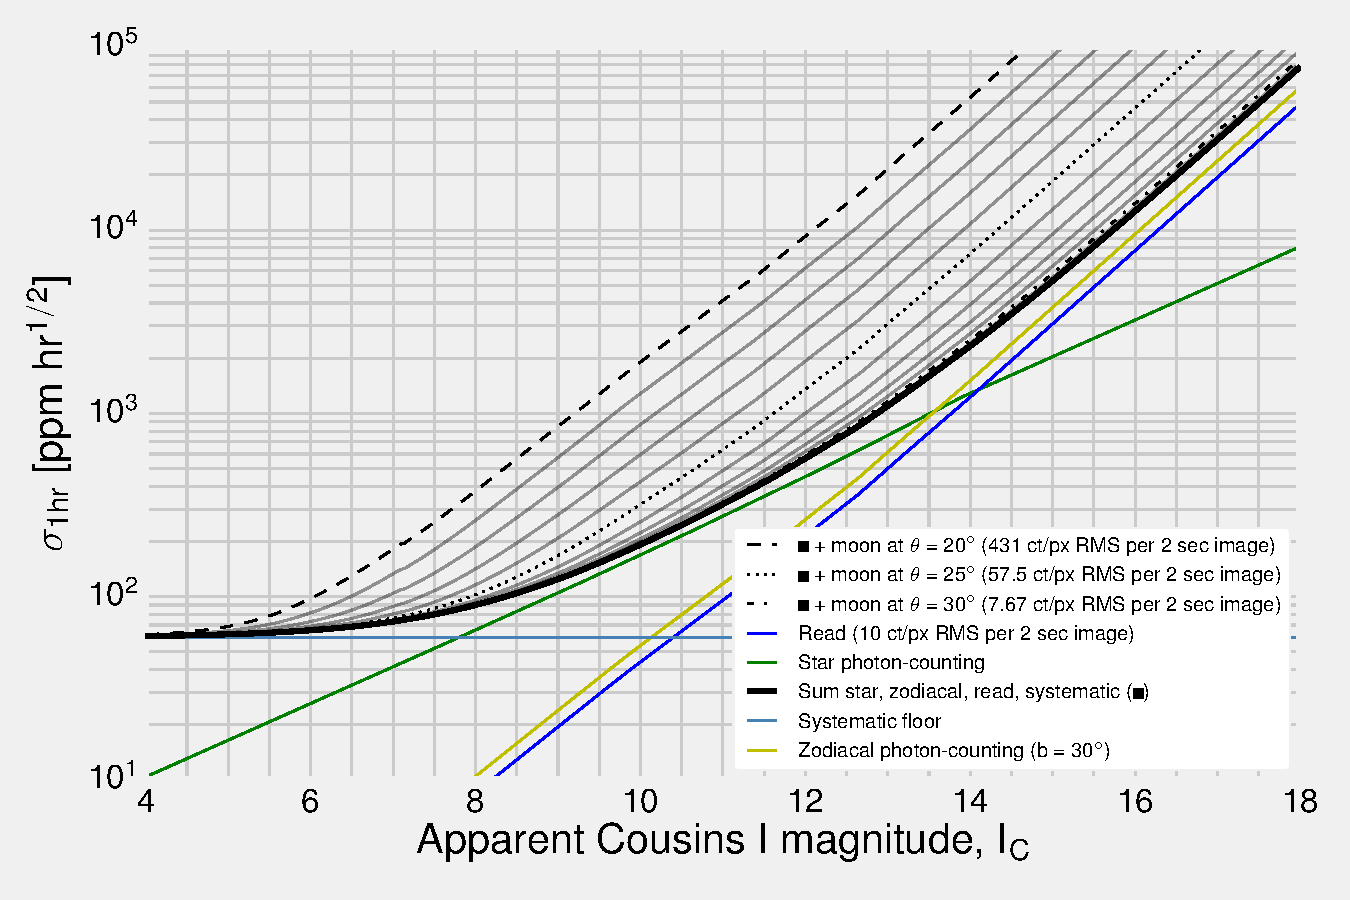
\includegraphics{figures/precision_angles_moon.pdf}
	\caption{Same as Fig.~\protect\ref{fig:sun_scat}, for scattered Moonlight.} 
	\label{fig:moon_scat}
\end{figure}
\begin{figure}[!t]
	\centering
	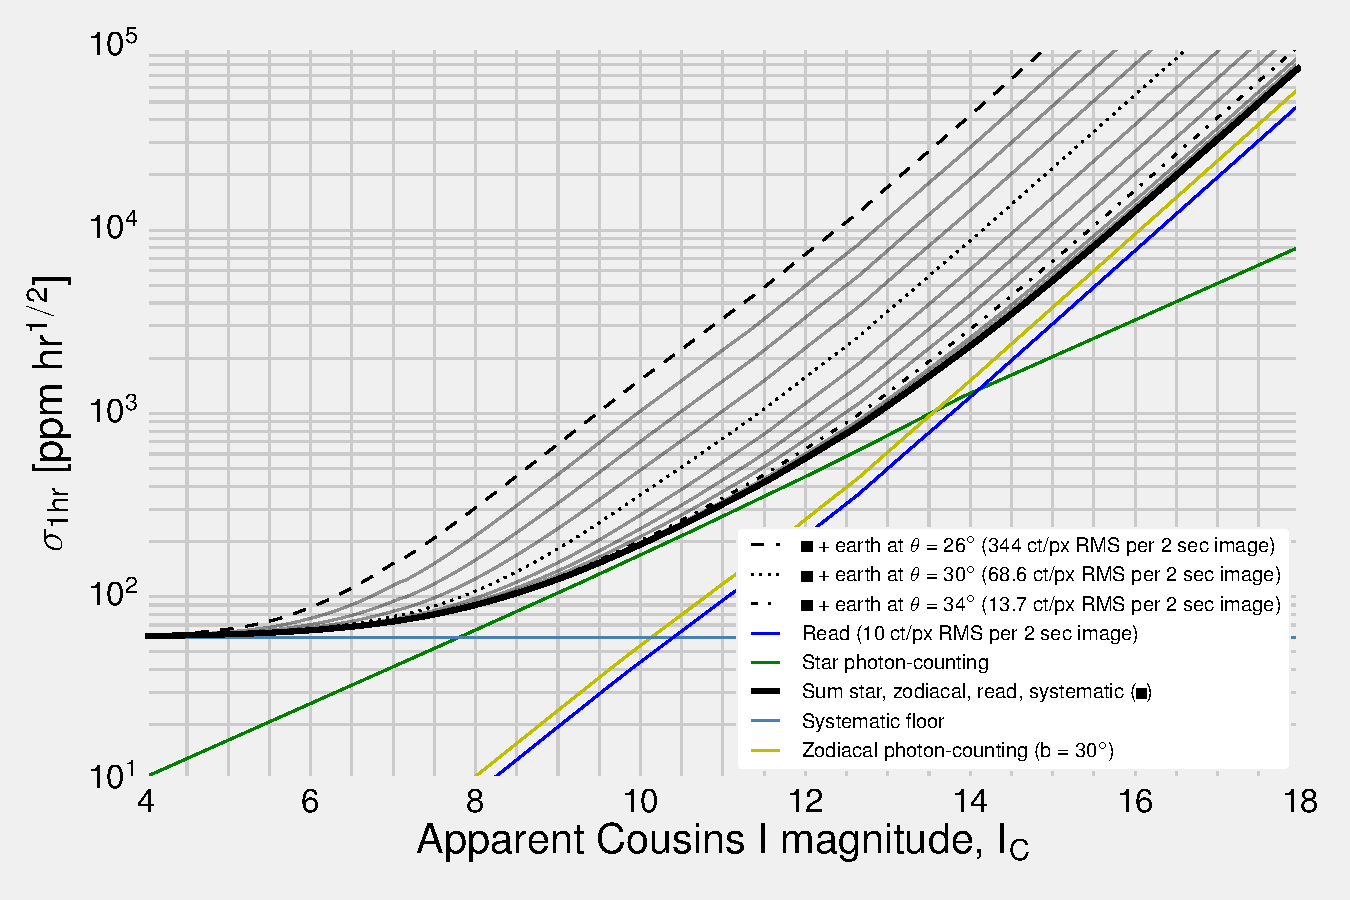
\includegraphics{figures/precision_angles_earth.pdf}
	\caption{Same as Fig.~\protect\ref{fig:sun_scat}, for scattered 
	Earthlight.} 
	\label{fig:earth_scat}
\end{figure}